\documentclass{article}
\usepackage[margin=1in]{geometry}
\usepackage{amsmath,amssymb}
\usepackage{verbatim}
\usepackage{graphicx}
\usepackage{xcolor,colortbl}
\usepackage[]{algorithm2e}
%\usepackage{cite}
\usepackage{caption}
\usepackage{mdframed}
\usepackage{float}
\setcounter{tocdepth}{5}
%\usepackage{soul}


\usepackage[backend=bibtex]{biblatex}
\addbibresource{bibliography.bib}


\newcommand{\red}[1]{\textbf{\color{red}{#1}}}

\newcommand{\tab}{\hspace{10mm}}
\newcommand{\dtab}{\hspace{20mm}}
\newcommand{\ttab}{\hspace{30mm}}
\newcommand{\qtab}{\hspace{40mm}}

\begin{document}

\title{Autonomous Agents 1 \\ Assignment 3}

\author{By Group 4: Gieske, Gornishka, Koster, Loor}
\maketitle

\pagebreak
\tableofcontents


\pagebreak

\section{Introduction}
This report contains the analysis of an implementation of multi-agent reinforcement learning. In this case, there can be multiple predators and there is one prey that needs to be caught. The predators all receive a positive reward of 10 if the prey is caught and the prey receives a negative reward of 10. However, if multiple predators bump into one another, they get confused and the prey gets away. In that case, the prey receives a positive reward of 10 and all predators receive a negative reward of 10. 

In this case, all agents learn using model-free learning. Three different ways of model-free learning are used: independent Q-learning, minimax Q-learning and independent SARSA. Though the workings of these methods have been researched extensively in the past, the prey never learned. Now this is different, which makes the game more interesting. Also, it is interesting to see if and how the predators are going to work together in order to catch the prey. Therefore, this paper focuses on the effects of these methods, implemented on all agents. Also, the effects of different parameter settings (learning rate, discount factor and $\epsilon$) are researched.


\pagebreak

\section{Theory}

\subsection{Independent Q-learning}
In independent Q-learning, all agents independently use Q-learning to maximize their expected reward.  \\ 

\noindent Q-learning\footnote{More specifically, this is \textit{one-step Q-learning}, which is the algorithm evaluated in this paper.} itself is a temporal difference method that uses the update rule in equation \eqref{eq:qupdate}. Since the algorithm retrieves the Q-value of the state-action pair where Q(s', a) is maximized, this is an \textit{off-policy} method. The algorithm for Q-learning can be found in pseudocode in figure \ref{alg:qlearning}.

\begin{mdframed}
\begin{align}
Q(s_t, a_t) \leftarrow Q(s_t,a_t) + \alpha \left[ r_{t+1} + \gamma \underset{a}{\text{max}} Q(s_{t+1},a) - Q(s_t,a_t)\right]\label{eq:qupdate}
\end{align}
\end{mdframed}


\begin{center} 
\begin{mdframed}
\begin{algorithm}[H]
Initialize Q(s,a) arbitrarily \\
Repeat (for each episode):\\
\tab Initialize s \\
\tab Repeat (for each step of episode):\\
\dtab Choose a from s' using policy derived from Q (e.g., $\epsilon$-greedy)\\
\dtab Take action a, observe r, s'\\
\dtab Q(s,a) $\leftarrow$ Q(s,a) + $\alpha [ r + \gamma \max_a' Q(s', a') - Q(s, a) ]$  \\
\dtab s $\leftarrow$ s'; \\
\tab until s is terminal\\
\end{algorithm}
\end{mdframed}
\captionof{figure}{The algorithm for one-step Q-learning\cite{bartosutton}}
\label{alg:qlearning}
\end{center}


\subsection{Independent Sarsa}
In independent SARSA, all agents use SARSA independently to maximize their expected reward.  \\ 

\noindent SARSA is a temporal difference method, like Q-learning, that uses the update rule in equation \ref{eq:supdate}. Because this algorithm retrieves the Q value after taking an $\epsilon$-greedy action, it is an \textit{on-policy} method. The algorithm for SARSA can be found in figure \ref{alg:slearning}.

\begin{mdframed}
\begin{align}
Q(s_t, a_t) \leftarrow Q(s_t,a_t) + \alpha \left[ r_{t+1} + \gamma Q(s_{t+1},a_{t+1}) - Q(s_t,a_t)\right]\label{eq:supdate}
\end{align}
\end{mdframed}


\begin{center}
\begin{mdframed}
\begin{algorithm}[H]
Initialize Q(s,a) arbitrarily\\
Repeat (for each episode):\\
\tab Initialize s \\
\tab Choose a from s' using policy derived from Q (e.g., $\epsilon$-greedy)\\
\tab Repeat (for each step of episode):\\
\dtab Take action a, observe r, s'\\
\dtab Choose a' from s' using policy derived from Q (e.g., $\epsilon$-greedy)\\
\dtab Q(s,a) $\leftarrow$ Q(s,a) + $\alpha [ r + \gamma Q(s', a') - Q(s, a) ]$ \\
\dtab s $\leftarrow$ s'; \\
\tab until s is terminal\\
\end{algorithm}
\end{mdframed}
\captionof{figure}{The algorithm for Sarsa \cite{bartosutton}}
\label{alg:slearning}
\end{center}


\subsection{Minimax Q-Learning} 
The problem with independent Q-learning is that it is based on a stationary environment, i.e. where the rules stay the same. However, in a Multi-agent environment where other agents learn as well, the environment is dynamic. This means that the guarantees that hold for single-agent learning do not hold in this setting. Littman \cite{Littman94markovgames} specifically considers two-player zero-sum games. In this type of Markov Game, it is possible to use a single reward function, that one player tries to \textit{maximize}, and the other (the opponent) tries to \textit{minimize}. For MDPs, there is a policy $\pi$ that is optimal. However, for Markov Games, there is often no \textit{undominated} policy\footnote{If a policy is dominated, that means a better policy exists}. The solution to this is to pick a policy and estimate its value by assuming the opponent will take the actions that are worst for the agents, with regards to this policy. In short, minimax picks the policy that maximizes the agent's reward in the worst case. This optimal policy can be stochastic, as seen in the policy for \textit{rock, paper, scissors} (where the best policy is being unpredictable so you cannot be exploited). To find the optimal policy $\pi^*$, linear programming can be used, where the value of a state is
\begin{mdframed}
\begin{align}
V(s) &= \underset{\pi \in PD(A)}{\text{max}} \underset{o \in O}{\text{min}} \sum_{a\in A} Q(s,a,o) \pi_a
\end{align}
\end{mdframed}
and the best action is selected using the Q-values, computed by
\begin{mdframed}
\begin{align}
Q(s,a,o) &= R(s,a,o) + \gamma \sum_{s'} T(s,a,o,s') V(s')
\end{align}
\end{mdframed}
where T is the transition function for transitioning from state $s$ to state $s'$ if the agent picks action $a$ and the opponent picks action $o$. However, since $s$ followed by $s'$ after actions $a$ and $o$ happens with a probability $T(s,a,o,s')$, this function can be left out of the equation.\\

Consequently, each agent uses the following update rule:

\begin{mdframed}
\begin{align}
Q(s,a,o) & \leftarrow Q(s,a,o) + \alpha (R + \gamma V(s') - Q(s,a,o))
\end{align}
\label{ref:minimaxrule}
\end{mdframed}
Then, linear programming is used to find a policy $\pi$ so that
\begin{mdframed}
\begin{align}
\pi(s,) \leftarrow \underset{\pi'(s,)}{\text{argmax }} \left\{ \underset{o'}{\text{min}} \left\{ \sum_{a'}  \left\{ \pi(s,a') \times Q(s,a',o') \right\} \right\} \right\}
\end{align}
\end{mdframed}

Eventually, the update rules can be used to implement the minimax-Q algorithm as described in figure \ref{alg:minmax}.

\begin{center} 
\begin{mdframed}
\begin{algorithm}[H]
Initialize Q(s,a) arbitrarily \\
Repeat (for each episode):\\
\tab Initialize s \\
\tab Repeat (for each step of episode):\\
\dtab Choose a from s' using policy derived from Q (e.g., $\epsilon$-greedy)\\
\dtab Take action a, observe reward R, s' and opponent's action o\\
\dtab Q(s,a,o) $\leftarrow$ Q(s,a,o) + $\alpha $(R + $\gamma$ V(s') - Q(s,a,o))  \\
\dtab $\pi(s,) \leftarrow \underset{\pi'(s,)}{\text{argmax }} \left\{ \underset{o'}{\text{min}} \left\{ \sum_{a'}  \left\{ \pi(s,a') \times Q(s,a',o') \right\} \right\} \right\}$ \\
\dtab $ V(s) \leftarrow \underset{o'}{\text{min}} \left\{ \sum_{a'}  \left\{ \pi(s,a') \times Q(s,a',o') \right\} \right\}  $ \\
\dtab $\alpha \leftarrow \alpha \times decay$
\end{algorithm}
\end{mdframed}
\captionof{figure}{Minimax-Q learning\cite{Littman94markovgames}}
\label{alg:minmax}
\end{center}






\begin{comment}
Initialize:
For all s in S, a in A, and o in O,
Let Q[s,a,o] := 1
For all s in S,
Let V[s] := 1
For all s in S, a in A,
Let pi[s,a] := 1/|A|
Let alpha := 1.0
Choose an action:
With probability explor, return an action uniformly at random.
Otherwise, if current state is s,
Return action a with probability pi[s,a].
Learn:
After receiving reward rew for moving from state s to s’
via action a and opponent’s action o,
Let Q[s,a,o] := (1-alpha) * Q[s,a,o] + alpha * (rew + gamma * V[s’])
Use linear programming to find pi[s,.] such that:
pi[s,.] := argmaxfpi’[s,.], minfo’, sumfa’, pi[s,a’] * Q[s,a’,o’]ggg
Let V[s] := minfo’, sumfa’, pi[s,a’] * Q[s,a’,o’]gg
Let alpha := alpha * decay
\end{comment}


% Update which one is the `other leanring'
%\subsection{Friend-or-Foe}
%Friend-or-Foe Q-learning is a multi-agent reinforcement learning technique in which the agent identifies other agents as a 'friend' or a 'foe' . For 'friend' agents a coordination equilibrium is to be found, that is an equilibrium in which all players achieve their highest possible value. If the other agent is a 'foe' agent an adversarial equilibrium is to be found. This equilibrium has the property that the agent is not hurt by any change of the other agent. The algorithm is an adaption of the Nash-Q update rule as seen in equation \ref{eq:nashq}, where the $NashQ$ function is replaced by a function specified for friend (\ref{eq:friend}) or foe agents (\ref{eq:foe}). \\
\begin{mdframed}
\begin{align}
Q_{t+1}^j(s,a^1, \dots, a^n) = (1-\alpha)Q_t^j(,a^1, \dots, a^n )+ \alpha[r_t^j+\gamma NashQ_t^j(s, Q^1, \dots, Q^n)]\label{eq:nashq}
\end{align}
\end{mdframed}

If agent is friend:
\begin{mdframed}
\begin{align}
\max\limits_{a_1\in A_1} Q^i[s,a^1, \dots, a^n]\label{eq:friend}\\
\end{align}
\end{mdframed}

%\begin{mdframed}
%\begin{align}
%\max\limits_{\pi \in \product(A_i)} min\limits_{a_i \in A_i} Q^i[s,a^1, \dots, a^n]\ref{eq:foe}\\
%\end{align}
%\end{mdframed}



\pagebreak

\section{Implementation}

\subsection{New state space}
In the previous assignments, two agents participated in the game. A predator chased a prey, which hardly ever moved and didn't learn. Now, the both the predator and the prey move around on the grid. Both agents learn and it is possible to initialize the game with up to four predators. This leads to a total of five agents. Adding an agent to the game increases the state space exponentially, making computation of Q-learning very expensive. Combined with the fact that all algorithms need time to learn and that multiple experiments must be run for accuracy, the algorithms will be executed several thousand times. It is, therefore, essential to calculate results as quick as possible. This will speed up significantly using state space encoding. Instead of checking the entire grid per agent, the distance to each agent is calculated. Along these distances, the Q-values are evaluated and used to take an action. The Q-values will be updated, not longer needing to update the entire grid after taking an action. Using this technique, only part of the Q-values are updated, per agent. This saves a lot of time, compared to the previous implementation.

\subsection{Files}

The implementation consists of the following files:
\begin{description}
	\item[Agents\_new] \hfill \\ 
	This file contains implementions of the Agent class, the Prey class and the Predator class. Both the predator and the prey inherit functions of the Agent class. The Agent class contains functions any agent needs, such as a set of actions, a policy and other functions. As the predator is the agent this implementation focuses on, the predator class contains more functions than the predator class.
	
	\item[Helpers] \hfill \\ 
	This file contains many helper functions. These functions aid in computation and decision making, but cannot (and need not) be part of a specific class.
	
	\item[Other\_objects] \hfill \\ % uncertain about policy class description
	This file contains the Policy and Environment classes. The environment of the game as well as the rules are implemented in the Environment class. The Policy class contains the implementation of Q-Learning, Sarsa and $\epsilon$-greedy action selection and more functions that help in determining and optimizing a policy as well as choosing an action of this policy.
	\item[Newstate] \hfill \\ 
	This file contains the Game class as well as a demonstration function. The Game class instantiates the game, initialized the predator and the prey and assigns policies to these. The game is run N times and the result is printed. The demonstration function also performs independent Q-learning, minimax Q-learning and independent Sarsa. It uses $\epsilon$-greedy action selection. The results are printed in the command line and graphs are used for analysis.
\end{description}

\pagebreak


\section{Analysis}
This section discusses the results of the implementations. In order to display and compare results, graphs are used. The title describes which parameters are analysed and the legend shows which color represents which setting of said parameters. Contrary to previous reports, tests were run 5 times with 2000 episodes. Eventually, the results were averaged and used for analysis. In order to analyse the results, several default parameters were established, based on the previous assignments. These are:

\begin{itemize}
\item 2000 runs
\item 5 experiments
\item 2 predators
\item 0.9 discount factor ($\gamma$)
\item 0.5 learning rate ($\alpha$)
\item 0.1 epsilon ($\epsilon$)
\end{itemize}

When testing the implementation or parameters, only the parameter under test changes. All other parameters have the default value as described above.

\subsection{Independent Q-Learning}
This section analyses the effects of independent Q-learning, as well as different parameter settings for this learning method.
\subsubsection{1 predator vs. 1 prey}
To start off, it is interesting to see if the new environment can cope with the new learning method. As not much changed compared to the previous implementation, it is interesting to see if the implementation still behaves as expected.

\begin{center}
	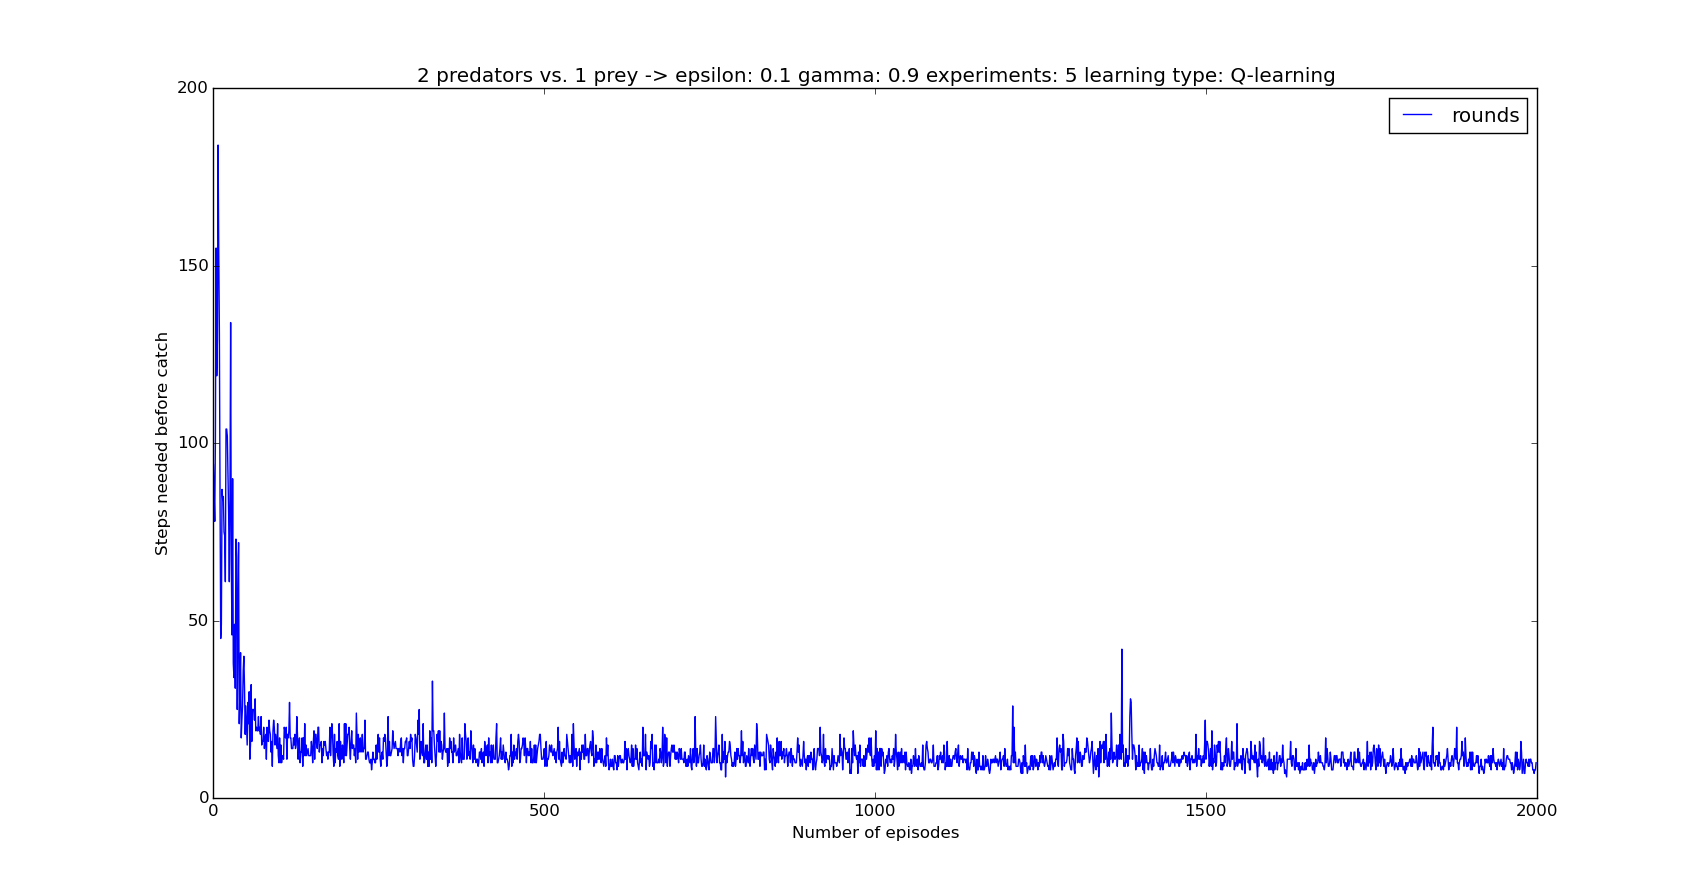
\includegraphics[scale=0.3]{1_predator_1_prey_q_learning}
	\captionof{figure}{Independent Q-learning: 1 predator vs. 1 prey}
\end{center}

As the graph shows, the predator learns how to catch the prey quicker after each time step. However, in the previous implementation, the number of time steps it took the predator to catch the prey became more stable. Though the number of time steps needed to catch the prey drops significantly, there is more variance than before. Also, the algorithm learns much quicker than before. As the state space grows exponentially larger with each added predator, the state space encoding was implemented to reduce the state space. Therefore, the each chosen action is always in the direction of the prey. This leads to catching the prey quicker than before as even the exploration steps bring the predator closer to the prey.

\subsubsection{2 predators vs. 1 prey}
Now there are two predators taking on one prey. The state space is now larger than before and leads to slower computation at each time step. Tests have shown that the amount of rounds it takes for any of the predators to catch the prey vary significantly. Therefore, the wins and losses of the predators have been taken into account, rather than the amount of rounds it takes the predators to catch the prey. However, the amount of rounds it takes does improve over time. Therefore, the number of rounds it takes the predators to catch the prey has been counted and is shown in the table below.

\begin{center}
	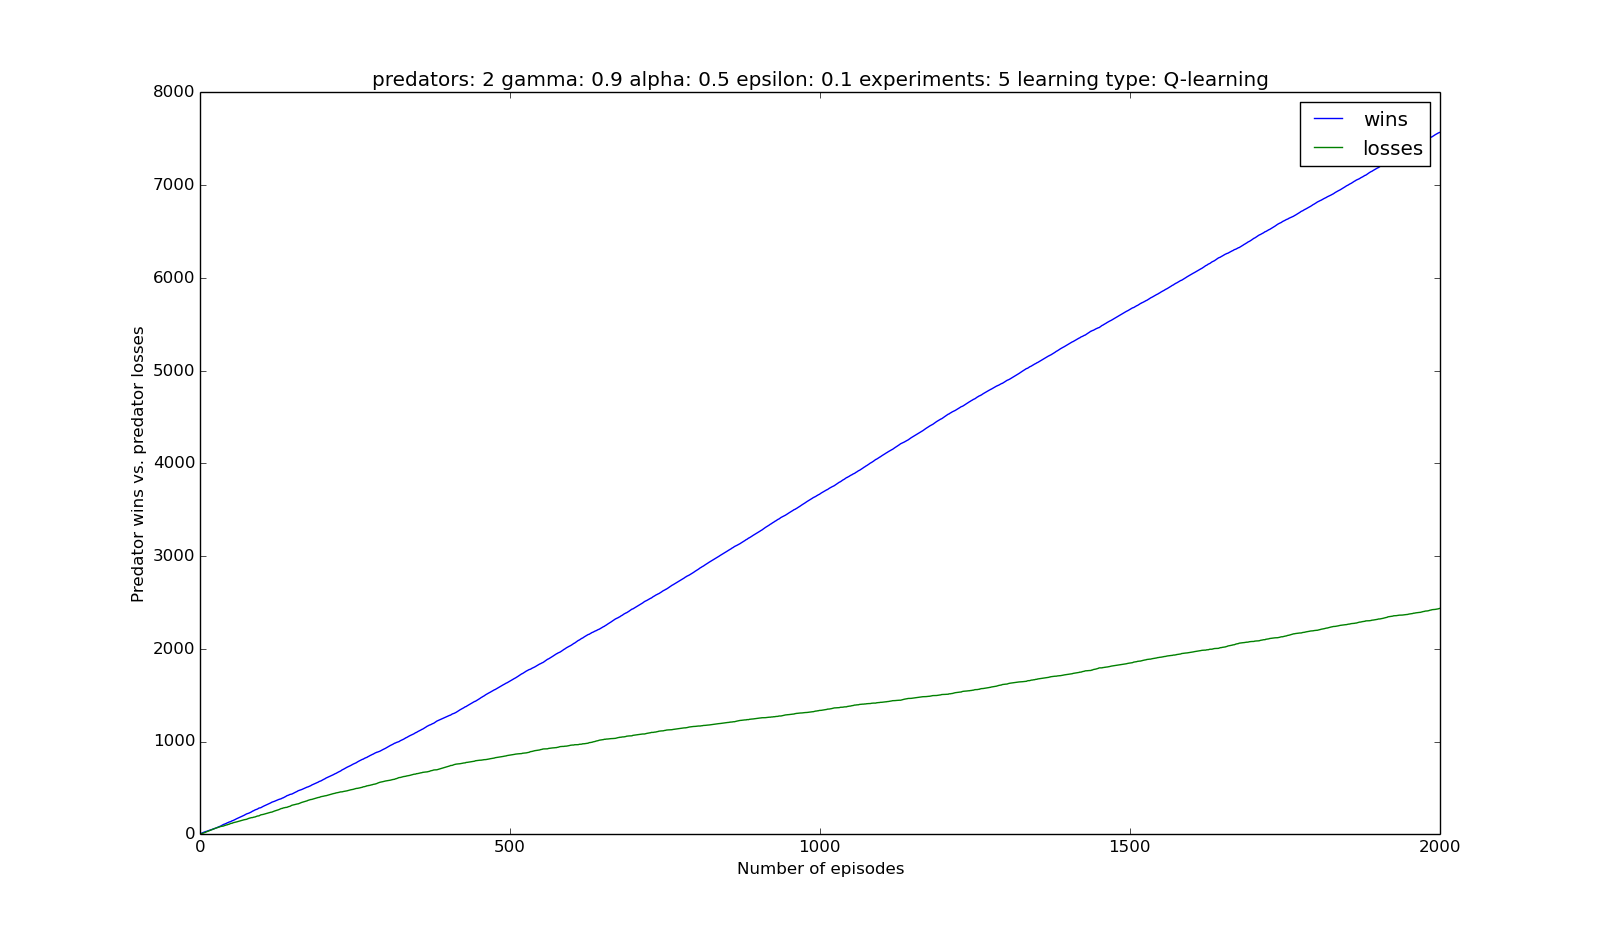
\includegraphics[scale=0.3]{2_predators_q_learning}
	\captionof{figure}{Independent Q-learning: 2 predators vs. 1 prey}
\end{center}

The graph shows that the predators learn to cooperate and catch the prey. This number increases, as the number of wins by the prey becomes less and less. As this is counted cumulatively, it can be expected that the number of wins by the prey will become almost steady. It is expected that, in the end, the predators will win almost each game. As their policies are still exploratory, it is possible for two predators to bump into one another and lose the game.

Now it is interesting to see whether or not the predators catch the prey in a certain amount of rounds.

\begin{table}[H]
\begin{center}
\begin{tabular}{| l | l | l | l | l |}
\hline
 & \parbox{2cm}{\textbf{Avg wins \\ (first 100)}} & \parbox{2cm}{\textbf{Avg losses \\ (first 100)}} & \parbox{2cm}{\textbf{Avg wins \\ (last 100)}} & \parbox{2cm}{\textbf{Avg losses \\ (last 100)}} \\
\hline
\textbf{Predators} & 58 & 42 & 76 & 23 \\
\hline
\end{tabular}
\caption{Average \# wins and losses by the predators}
\end{center}
\end{table}

As the table shows, the predators learn to catch the prey quicker over time.

\subsubsection{3 predators vs. 1 prey}
By placing four agents on the grid, the implementation became very slow. It was possible to run the implementation, but as it is very slow, the parameter changes have not been tested. However, figure -some-reference- shows the results of 3 predators vs. one prey.

This figure shows that the predators lose the game a lot. This is interesting as it is expected of the predators to learn not to bump into one another. However, the grid is both toroidal as well as small and the prey learns. It is possible that the prey learning, combined with a small, toroidal grid, leads to the predators bumping into one another. Perhaps the prey learns to trick the predators into bumping into one another. Therefore, it is interesting to see what happens if the prey learns slower than the predators. By making the prey learn slower, theoretically it is possible for the predators to learn not to bump into one another and catch the prey. 

\subsubsection{4 predators vs. 1 prey}
Though it is implemented for four predators and one prey to be placed on the grid, this leads to implementations freezing. It is therefore conclusive to state that the program has become intractable. 

\subsubsection{Parameter settings}
It is interesting to see what happens when the parameters of the learning methods change. As the effects parameter settings have been researched in a 1 vs. 1 scenario, it is interesting to see what is different when there are more agents on the grid. Also, as all agents now learn, the effects of these learning methods should change.

\subsubsection{Learning rate}
First, the effect of the learning rate is researched. As the learning rate determines to what extent the newly acquired information will override the old information, it is interesting to see what happens. 

\begin{center}
	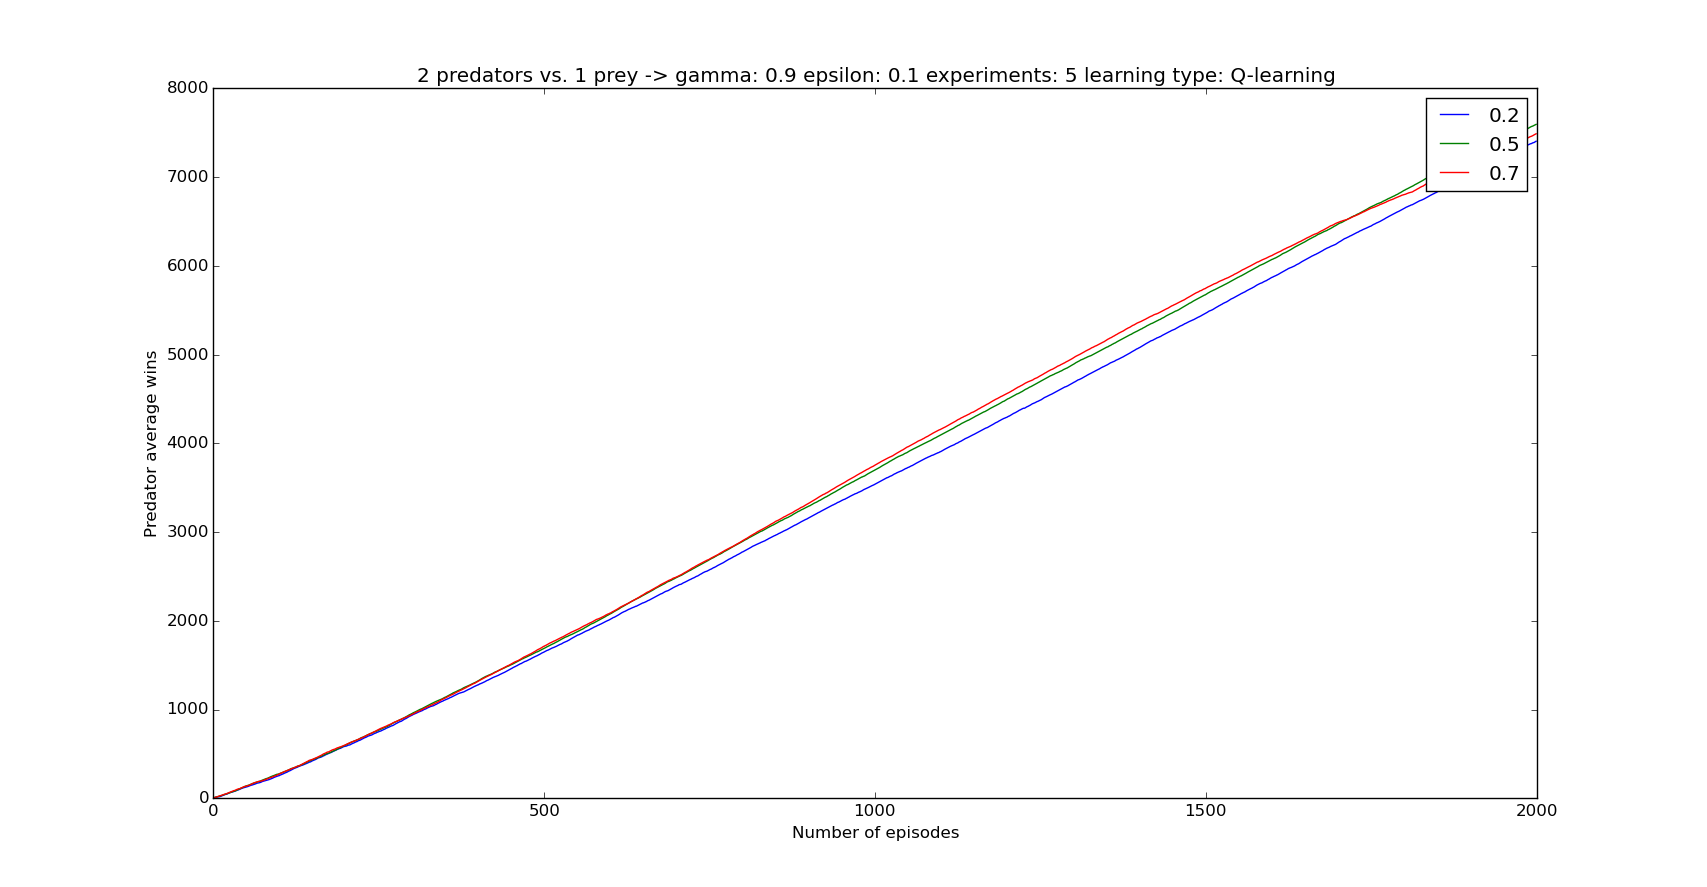
\includegraphics[scale=0.3]{2_predators_learning_rate_q_learning}
	\captionof{figure}{Independent Q-learning: 2 predators vs. 1 prey, learning rate}
\end{center}

From the graph it is easy to see that a low learning rate yields worst results. For a long time, a high learning rate yields good results, however, in the end a learning rate of 0.5 yields best results. This shows that for a long time, a lot of recent information is interesting.  Later on, however, an even balance of new and old information leads to more wins for the predator. 

\begin{table}[H]
\begin{center}
\begin{tabular}{| l | l | l | l | l |}
\hline
\parbox{2cm}{\textbf{Learning rate}} & \parbox{2cm}{\textbf{Avg wins \\ (first 100)}} & \parbox{2cm}{\textbf{Avg losses \\ (first 100)}} & \parbox{2cm}{\textbf{Avg wins \\ (last 100)}} & \parbox{2cm}{\textbf{Avg losses \\ (last 100)}} \\
\hline
\textbf{0.2} & 50 & 49 & 74 & 24 \\
\hline
\textbf{0.5} & 54 & 45 & 72 & 27 \\
\hline
\textbf{0.7} & 54 & 45 & 63 & 35 \\
\hline
\end{tabular}
\caption{Average \# wins and losses by the predators with varying learning rates}
\end{center}
\end{table}

The table shows that the lowest learning rate shows better and better results over time. This shows that in the beginning, a lot must be learned. As the game progresses, the prey becomes less predictable and a low learning rate yields better results. This could indicate that the predators as well as the prey become predictable and so less has to be learned about them. As minimax Q-learning contains a decay in learning, perhaps this is the reason why. %this is strange.

\subsubsection{Discount factor}
The discount factor determines the importance of future rewards. In the previous assignment, the a high discount factor yielded best results. This means that the future reward was most important. Only the goal state yielded a reward, making reaching the goal state very important. Currently, there are two terminal states: the win state and the lose state. It is interesting to see what effect the negative rewards have on the importance of the immediate reward.

\begin{center}
	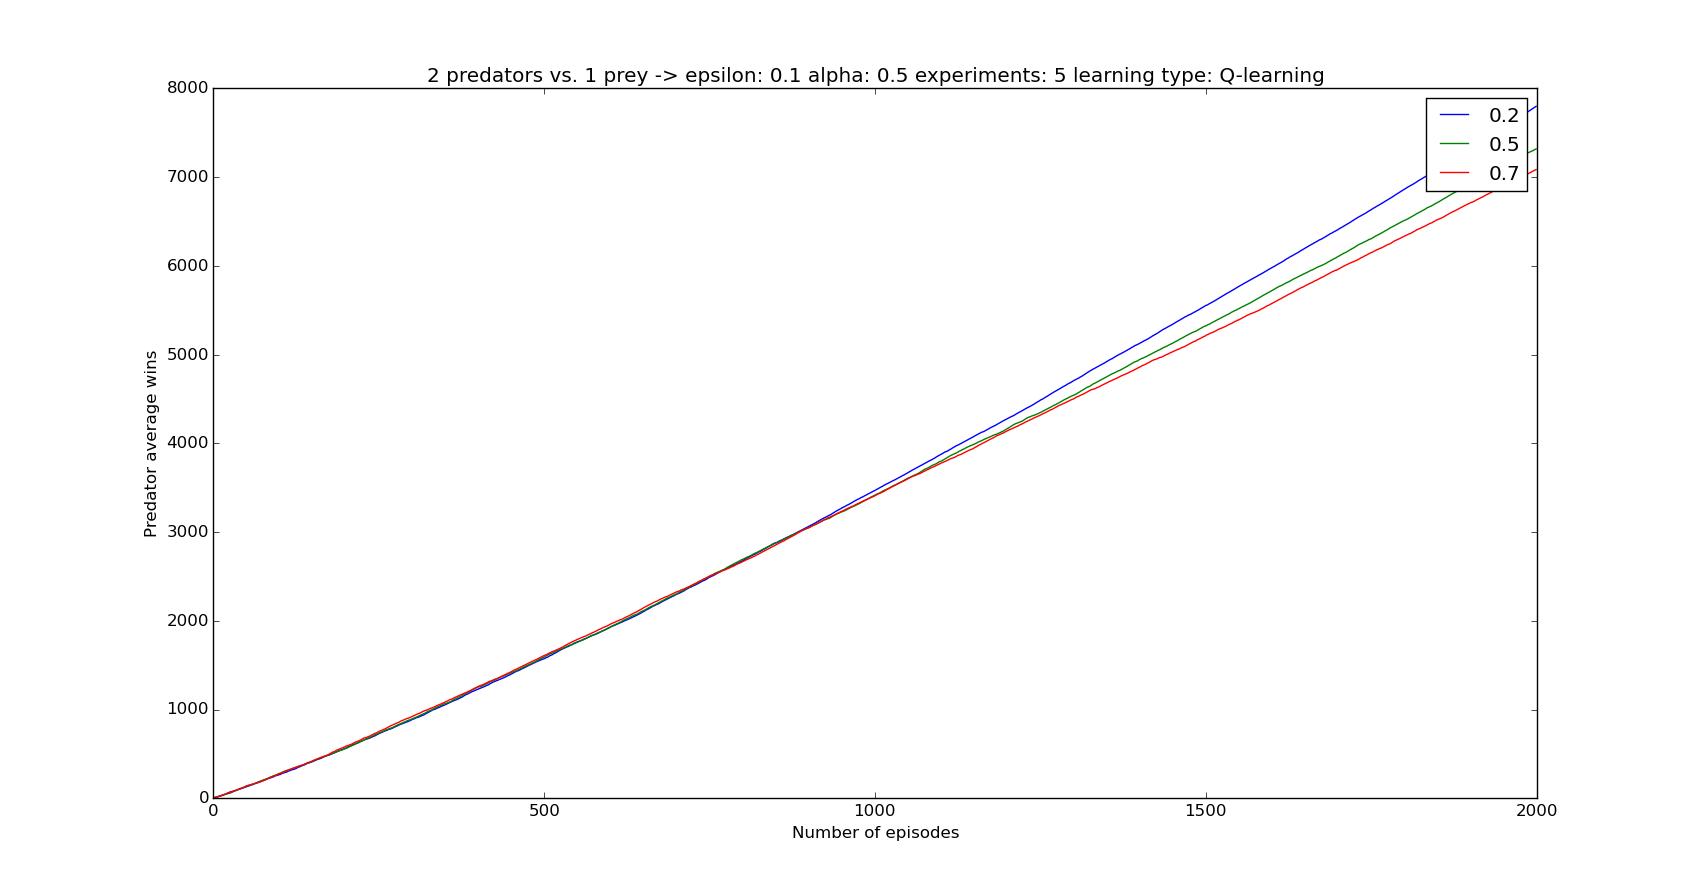
\includegraphics[scale=0.3]{2_predators_discount_factor_q_learning}
	\captionof{figure}{Independent Q-learning: 2 predators vs. 1 prey, discount factor}
\end{center}

The graph shows that for a long time, it does not matter how important the future reward is. However, eventually the graph shows that a low discount factor yields best results. This can be caused by the fact that the predators will receive a negative reward when running into another predator. In order to avoid this, the immediate reward has to become more important.

\begin{table}[H]
\begin{center}
\begin{tabular}{| l | l | l | l | l |}
\hline
\parbox{2cm}{\textbf{Discount factor}} & \parbox{2cm}{\textbf{Avg wins \\ (first 100)}} & \parbox{2cm}{\textbf{Avg losses \\ (first 100)}} & \parbox{2cm}{\textbf{Avg wins \\ (last 100)}} & \parbox{2cm}{\textbf{Avg losses \\ (last 100)}} \\
\hline
\textbf{0.2} & 52 & 47 & 98 & 4 \\
\hline
\textbf{0.5} & 55 & 44 & 78 & 21 \\
\hline
\textbf{0.7} & 55 & 45 & 74 & 24 \\
\hline
\end{tabular}
\caption{Average \# wins and losses by the predators with varying discount factors}
\end{center}
\end{table}

The table shows that the discount factor has a huge impact on the success of the predators. By making sure that the predators do not run into each other, the game is less often lost.

\subsubsection{$\epsilon$-greedy action selection}
Selecting the next action is important. There has to be a balance between exploration and exploitation. One of the most widely used techniques is $\epsilon$-greedy action selection. That is also the action selection method used in this case. This is where the $\epsilon$ factor comes into action. This factor determines how greedy the action selection is. An $\epsilon$ value of 0 selects only greedy actions. The closer this values is to 1, the more exploring actions are selected. The following figure shows the results of this test.

\begin{center}
	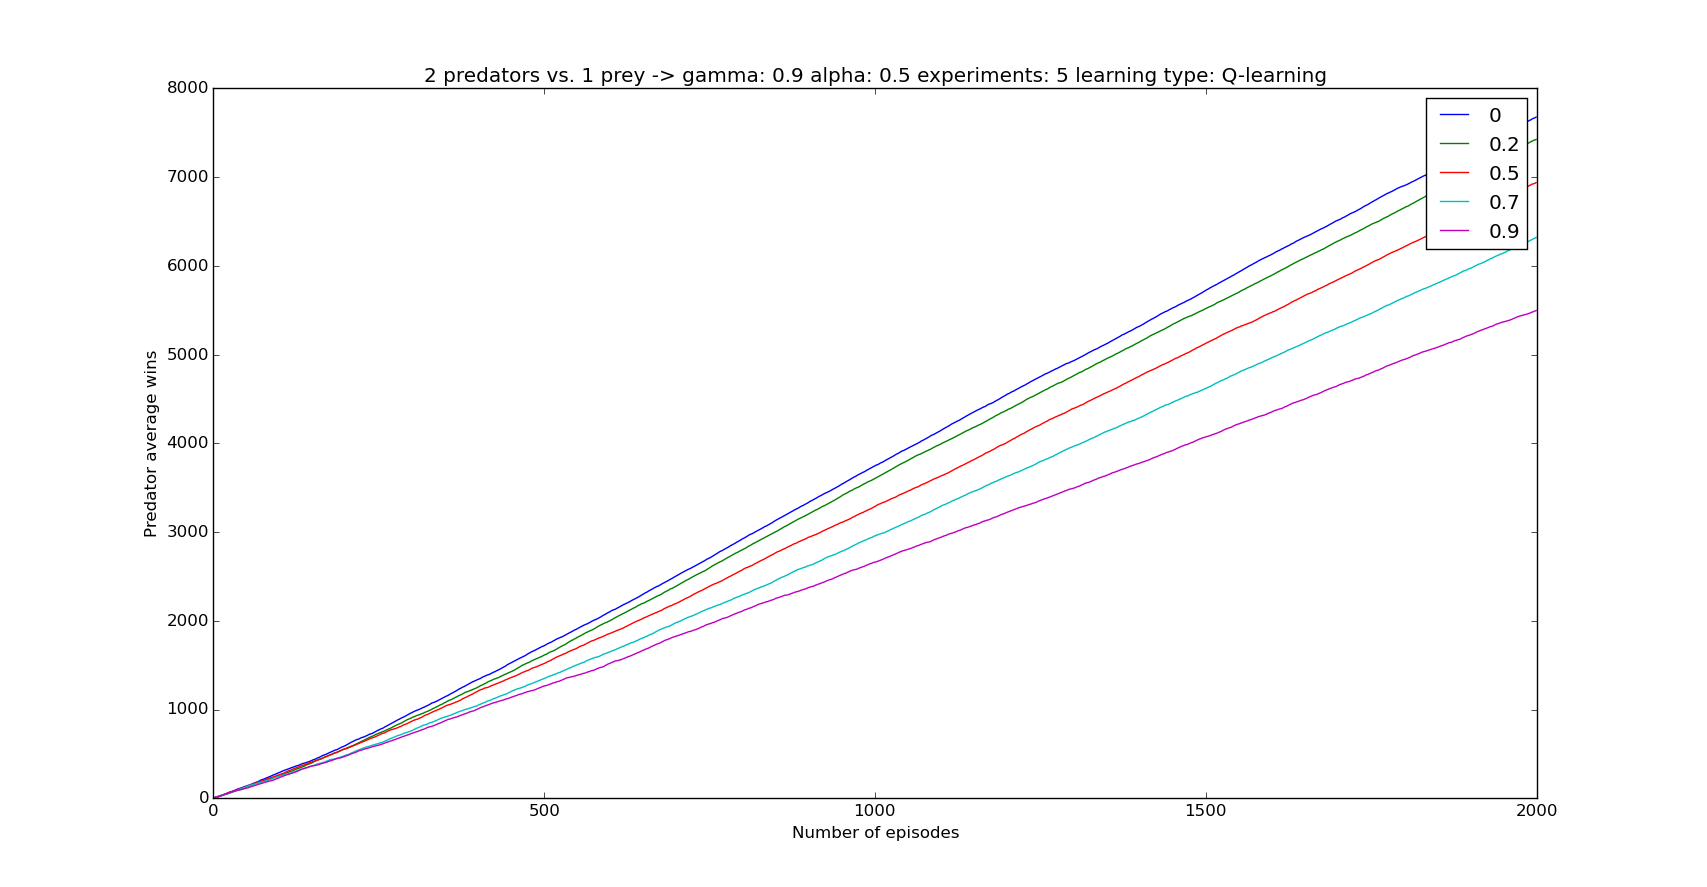
\includegraphics[scale=0.3]{2_predators_epsilon_q_learning}
	\captionof{figure}{Independent Q-learning: 2 predators vs. 1 prey, $\epsilon$-greedy action selection}
\end{center}

Figure \# shows that greedy action selection yields best results. This is possible, as all predators are initialized at the corners of the grid, starting out with equal distance to the prey. As the prey moves, it will be closer to one predator. Therefore, without exploration, the prey will be caught by one predator. As a greedy action, in this case, leads to moving in the direction of the highest Q-value, it is still possible for the predators to bump into each other. However, it seems as if the prey is most often caught before this happens leading to wins for the predators.

\begin{table}[H]
\begin{center}
\begin{tabular}{| l | l | l | l | l |}
\hline
\parbox{2cm}{\textbf{$\epsilon$-rate}} & \parbox{2cm}{\textbf{Avg wins \\ (first 100)}} & \parbox{2cm}{\textbf{Avg losses \\ (first 100)}} & \parbox{2cm}{\textbf{Avg wins \\ (last 100)}} & \parbox{2cm}{\textbf{Avg losses \\ (last 100)}} \\
\hline
\textbf{0} & 55 & 44 & 76 & 22 \\
\hline
\textbf{0.2} & 54 & 45 & 77 & 21 \\
\hline
\textbf{0.5} & 49 & 50 & 72 & 27 \\
\hline
\textbf{0.7} & 48 & 51 & 66 & 32 \\
\hline
\textbf{0.9} & 50 & 59 & 55 & 44 \\
\hline
\end{tabular}
\caption{Average \# wins and losses by the predators with varying $\epsilon$-rates}
\end{center}
\end{table}

Though, at first, an absolute greedy policy appears to yield the most promising results, a slightly exploratory policy eventually yields the best results. This is not displayed in the graph as the wins are counted cumulatively. Eventually, the results will be best when still exploring sightly.

\subsection{Independent Sarsa}
This section discusses the effects of independent SARSA learning.
\subsubsection{1 predator vs. 1 prey}
Again, it is interesting to see if independent SARSA works well with the new environment. Te test this, the new environment executed a game of 1 predator vs. 1 prey. The results can be found in figure \#.

\begin{center}
	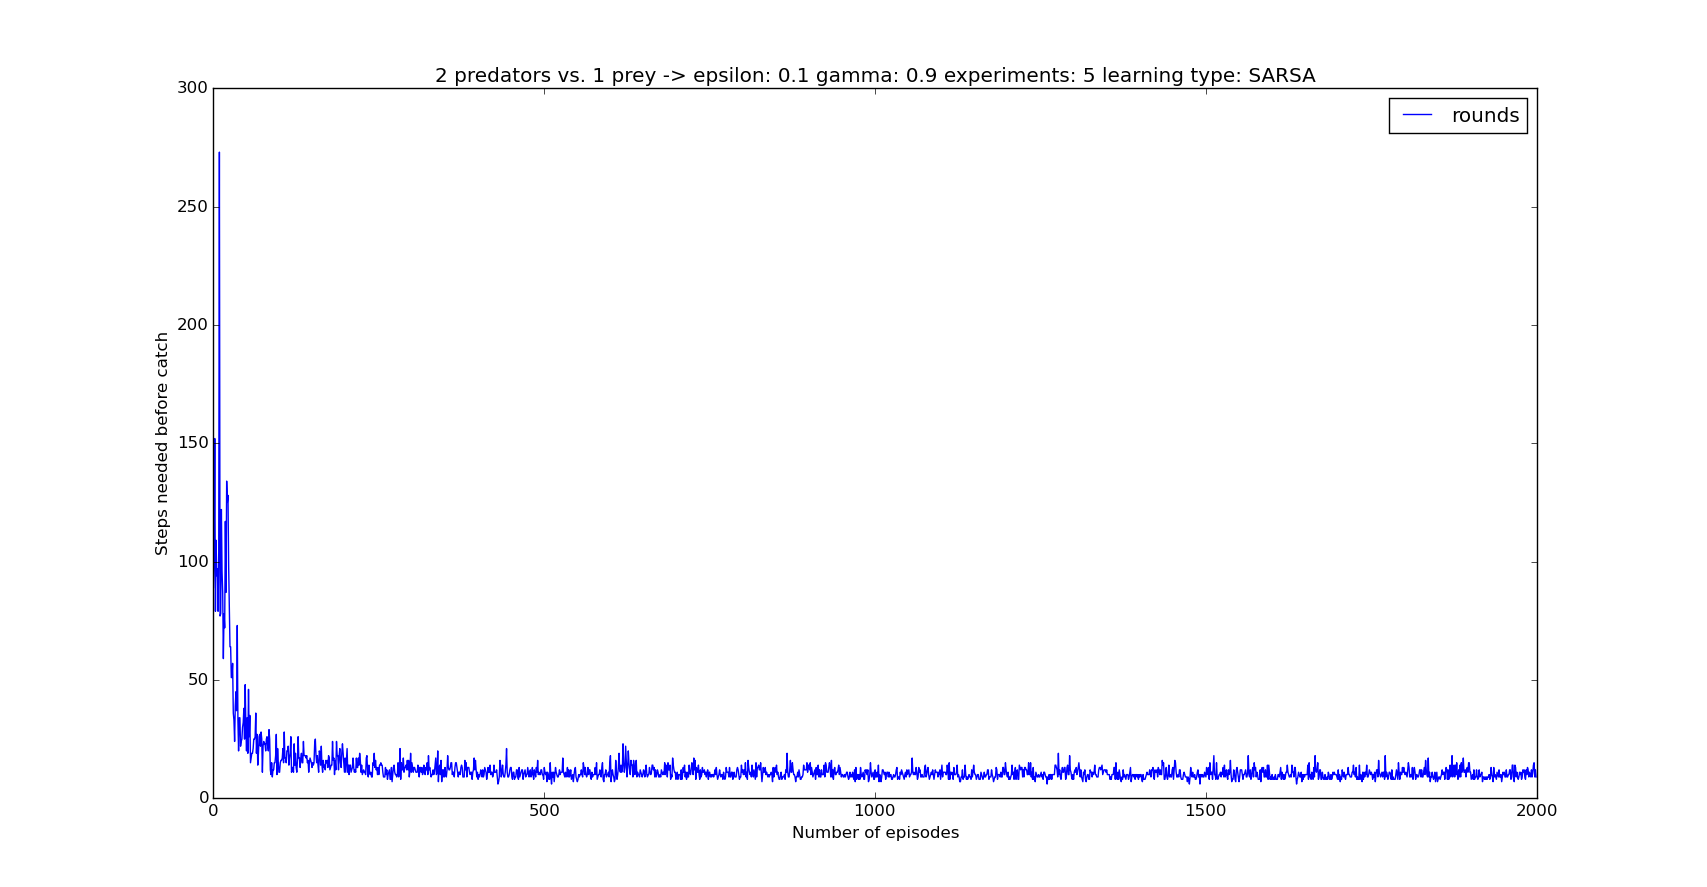
\includegraphics[scale=0.3]{1_predator_1_prey_SARSA}
	\captionof{figure}{Independent SARSA: 1 predator vs. 1 prey}
\end{center}

As seen with independent Q-learning, the predator learns how to catch the prey quicker than before. This confirms the theory that the smaller state space leads to quicker conversion of the algorithms. 

Compared to independent Q-learning, SARSA takes much longer to catch the prey in the beginning. Also, after learning the amount of rounds it takes the predators to catch the prey still vary much. However, where there is a spike rounds in Q-learning, there is not in SARSA. This happens due to the fact that SARSA is more careful than Q-learning. As SARSA is an on-policy learning algorithm, it is more careful than Q-learning. This leads to less extreme exploratory actions, choosing the "safe path" more often than Q-learning.

\subsubsection{2 predators vs. 1 prey}
\begin{center}
	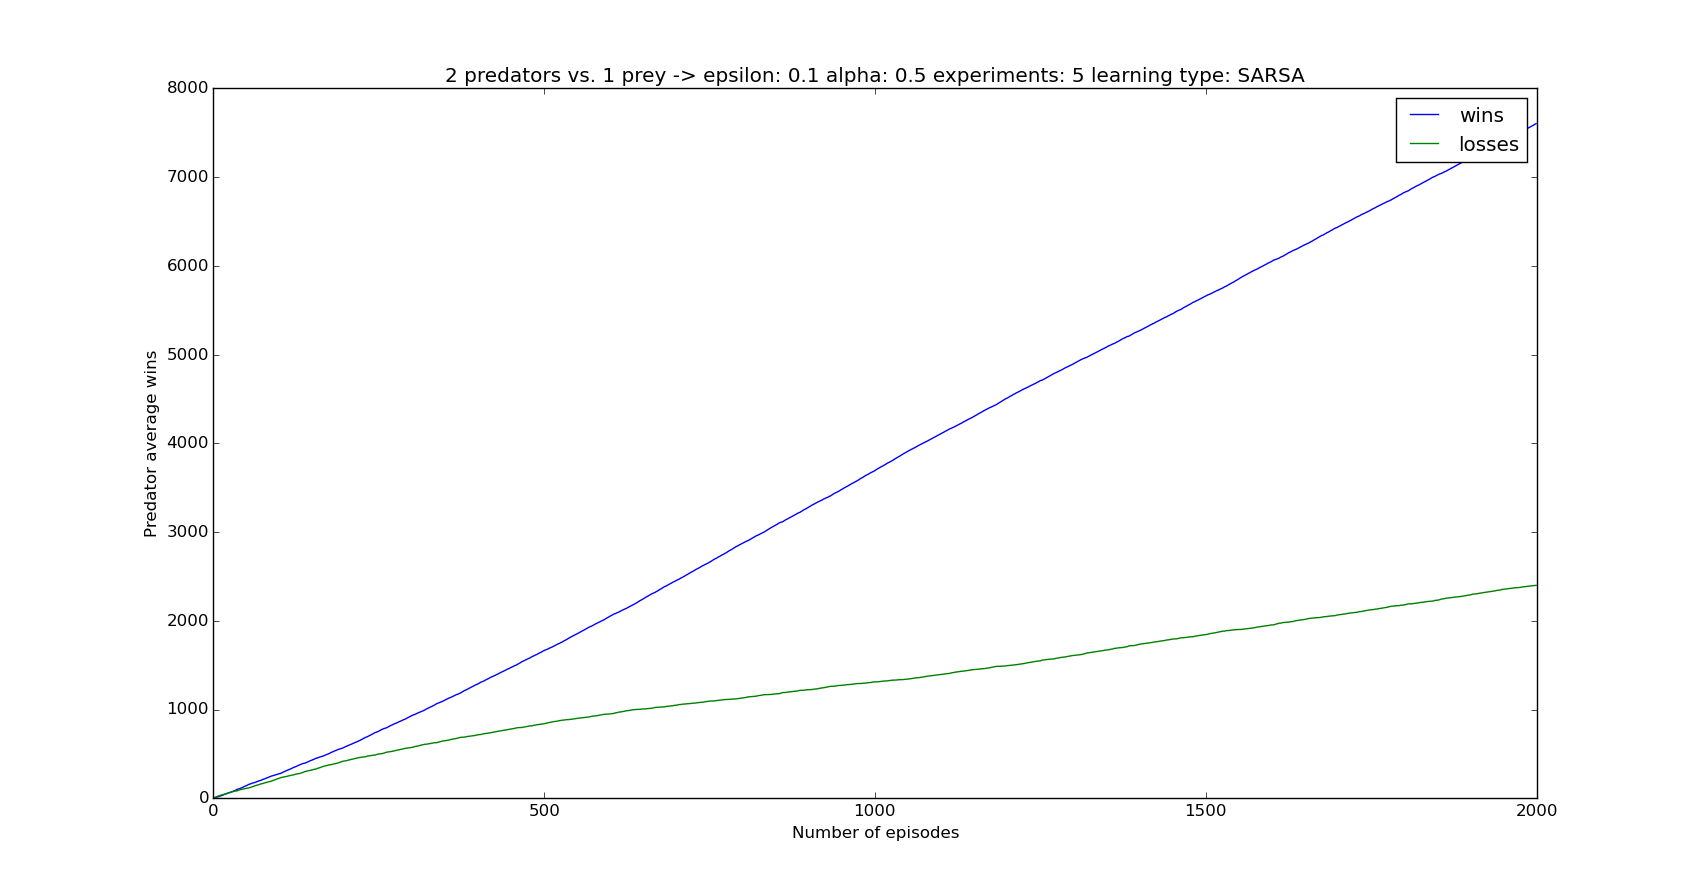
\includegraphics[scale=0.3]{2_predators_SARSA}
	\captionof{figure}{Independent SARSA: 2 predators vs. 1 prey}
\end{center}

The graph is very similar to the graph in Q-learning. This is possible, as both are temporal difference learning methods and are based on the same principles. The main difference between these two is that SARSA is an on-policy learning method and Q-learning is an off-policy learning method. It is therefore expected for these two methods to behave similarly.

\begin{table}[H]
\begin{center}
\begin{tabular}{| l | l | l | l | l |}
\hline
 & \parbox{2cm}{\textbf{Avg wins \\ (first 100)}} & \parbox{2cm}{\textbf{Avg losses \\ (first 100)}} & \parbox{2cm}{\textbf{Avg wins \\ (last 100)}} & \parbox{2cm}{\textbf{Avg losses \\ (last 100)}} \\
\hline
\textbf{Predators} & 55 & 44 & 78 & 21 \\
\hline
\end{tabular}
\caption{Average \# wins and losses by the predators}
\end{center}
\end{table}

Compared to independent Q-learning, independent SARSA performs slightly better. This can be attributed to the fact that SARSA is more careful than Q-learning. This behaviour leads to more wins for the predators, on average, compared to Q-learning.

\subsubsection{3 predators vs. 1 prey}
It is interesting to see what happens when three predators take on one prey. As seen with independent Q-learning, this does not work well. As SARSA is a more careful algorithm, the predators may learn to cooperate better than with Q-learning.

\begin{center}
	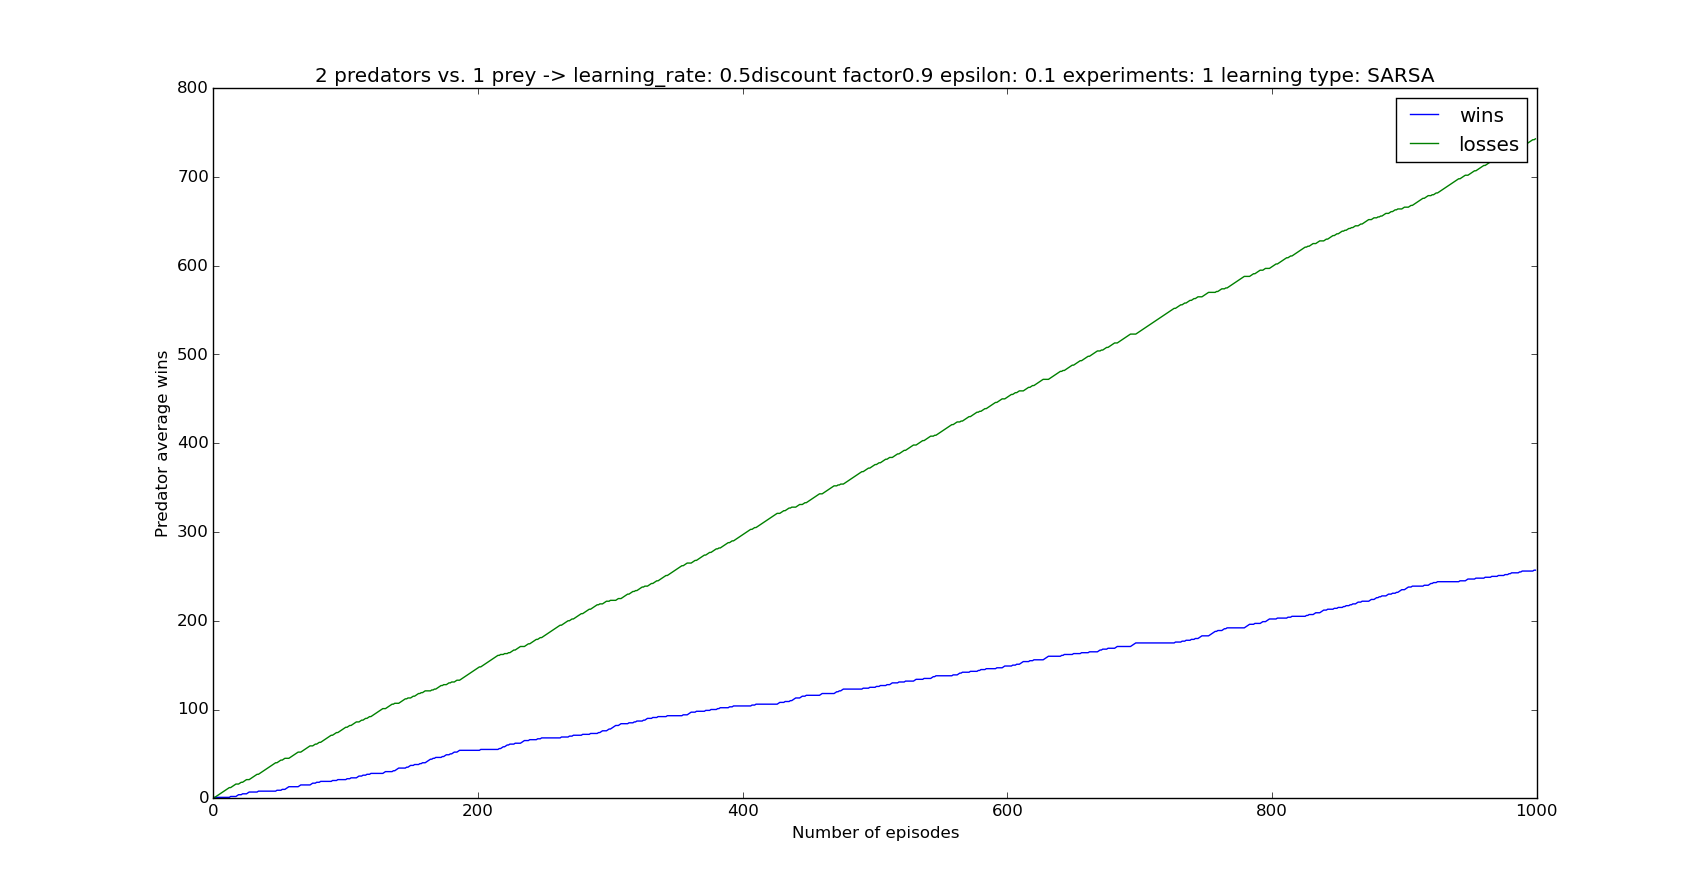
\includegraphics[scale=0.3]{3_predators_SARSA}
	\captionof{figure}{Independent SARSA: 3 predators vs. 1 prey}
\end{center}

The graph shows that the prey manages to escape most of the times. This hardly differs from independent Q-learning.

\begin{table}[H]
\begin{center}
\begin{tabular}{| l | l | l | l | l |}
\hline
 & \parbox{2cm}{\textbf{Avg wins \\ (first 100)}} & \parbox{2cm}{\textbf{Avg losses \\ (first 100)}} & \parbox{2cm}{\textbf{Avg wins \\ (last 100)}} & \parbox{2cm}{\textbf{Avg losses \\ (last 100)}} \\
\hline
\textbf{Predators} & 21 & 79 & 22 & 77 \\
\hline
\end{tabular}
\caption{Average \# wins and losses by the predators with varying learning rates}
\end{center}
\end{table}

This shows that SARSA learns very slowly, in this case. Combined with the fact that there are many predators on a small grid, these can bump into one another. Any learning will be much delayed. It is important to note that this is the only test which was run once, with 1000 episodes.

\subsubsection{4 predators vs. 1 prey}
Again, this is intractable. 

\subsubsection{Parameter settings}
Again, parameter settings were explored for this algorithm. This was tested with two predators and one prey.

\subsubsection{Learning rate}
First, the effect of the learning rate is researched. As the learning rate determines to what extent the newly acquired information will override the old information, it is interesting to see what happens. 

\begin{center}
	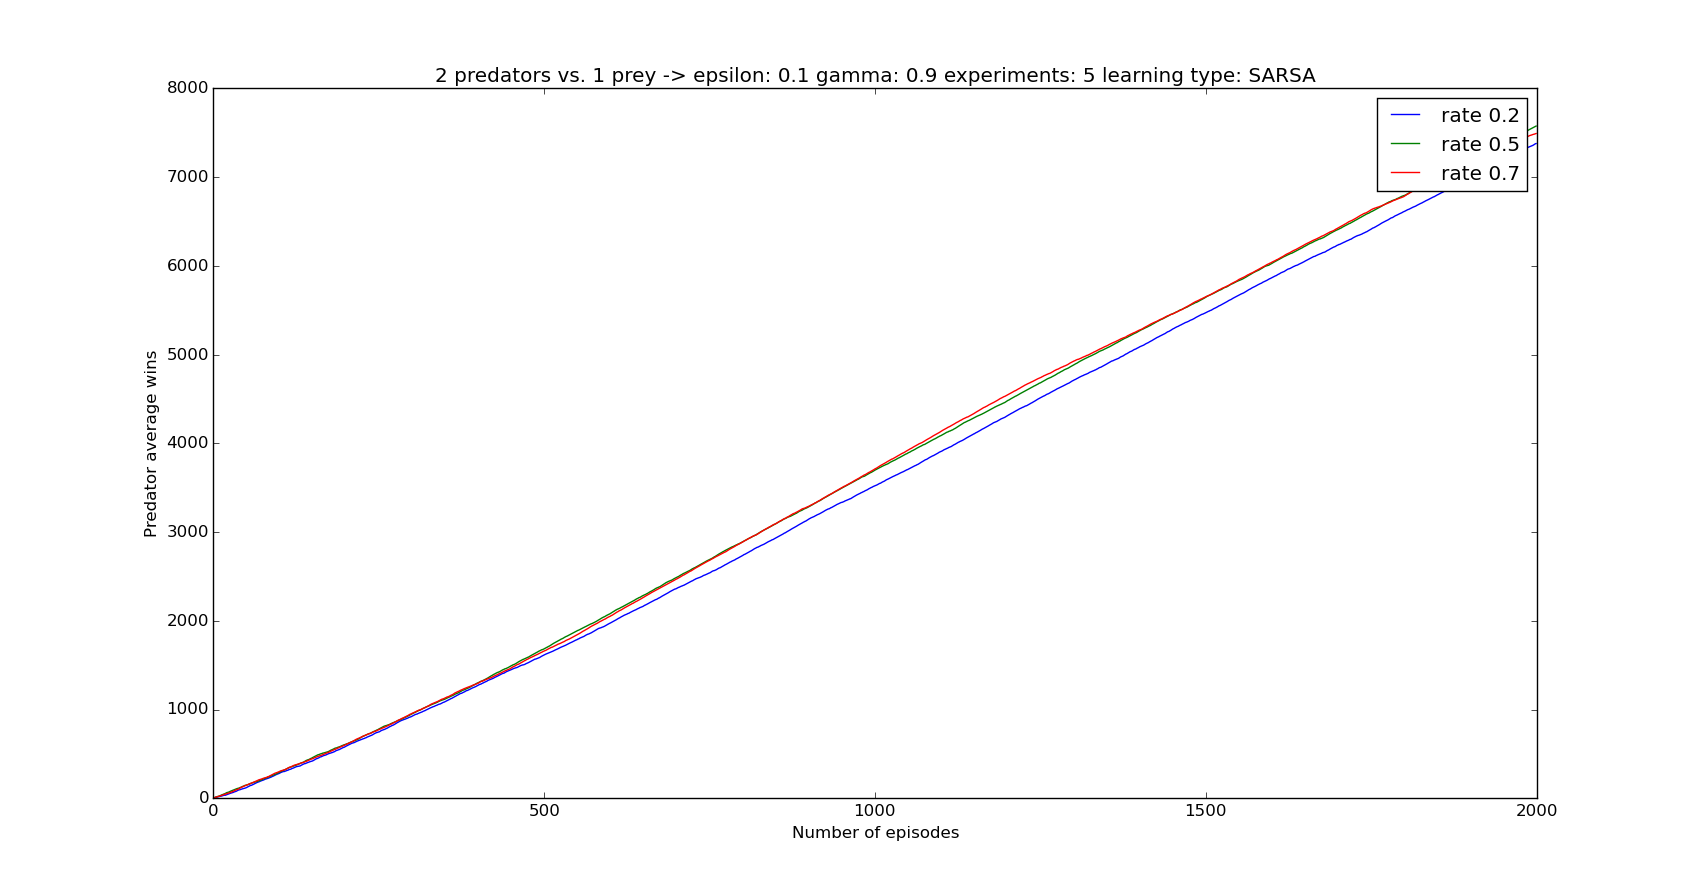
\includegraphics[scale=0.3]{2_predators_learning_rate_SARSA}
	\captionof{figure}{Independent SARSA: 2 predators vs. 1 prey, learning rate}
\end{center}

From the graph it is difficult to see if a high or average learning rate affect the implementation in the best possible way. In the end, however it appears as though a learning rate of 0.5 yields best results.

\begin{table}[H]
\begin{center}
\begin{tabular}{| l | l | l | l | l |}
\hline
\parbox{2cm}{\textbf{$\epsilon$-rate}} & \parbox{2cm}{\textbf{Avg wins \\ (first 100)}} & \parbox{2cm}{\textbf{Avg losses \\ (first 100)}} & \parbox{2cm}{\textbf{Avg wins \\ (last 100)}} & \parbox{2cm}{\textbf{Avg losses \\ (last 100)}} \\
\hline
\textbf{0.2} & 56 & 44 & 75 & 23 \\
\hline
\textbf{0.5} & 58 & 41 & 79 & 19 \\
\hline
\textbf{0.7} & 59 & 40 & 68 & 30 \\
\hline
\end{tabular}
\caption{Average \# wins and losses by the predators with varying learning rates}
\end{center}
\end{table}

The table confirms the theory derived off the graph. A learning rate does yield best results. When the predators are learning while hunting the prey, an equal balance of new and old information yields optimal results.

\subsubsection{Discount factor}
The discount factor determines the importance of future rewards. In the previous assignment, the a high discount factor yielded best results. This means that the future reward was most important. Only the goal state yielded a reward, making reaching the goal state very important. Currently, there are two terminal states: the win state and the lose state. It is interesting to see what effect the negative rewards have on the importance of the immediate reward.

\begin{center}
	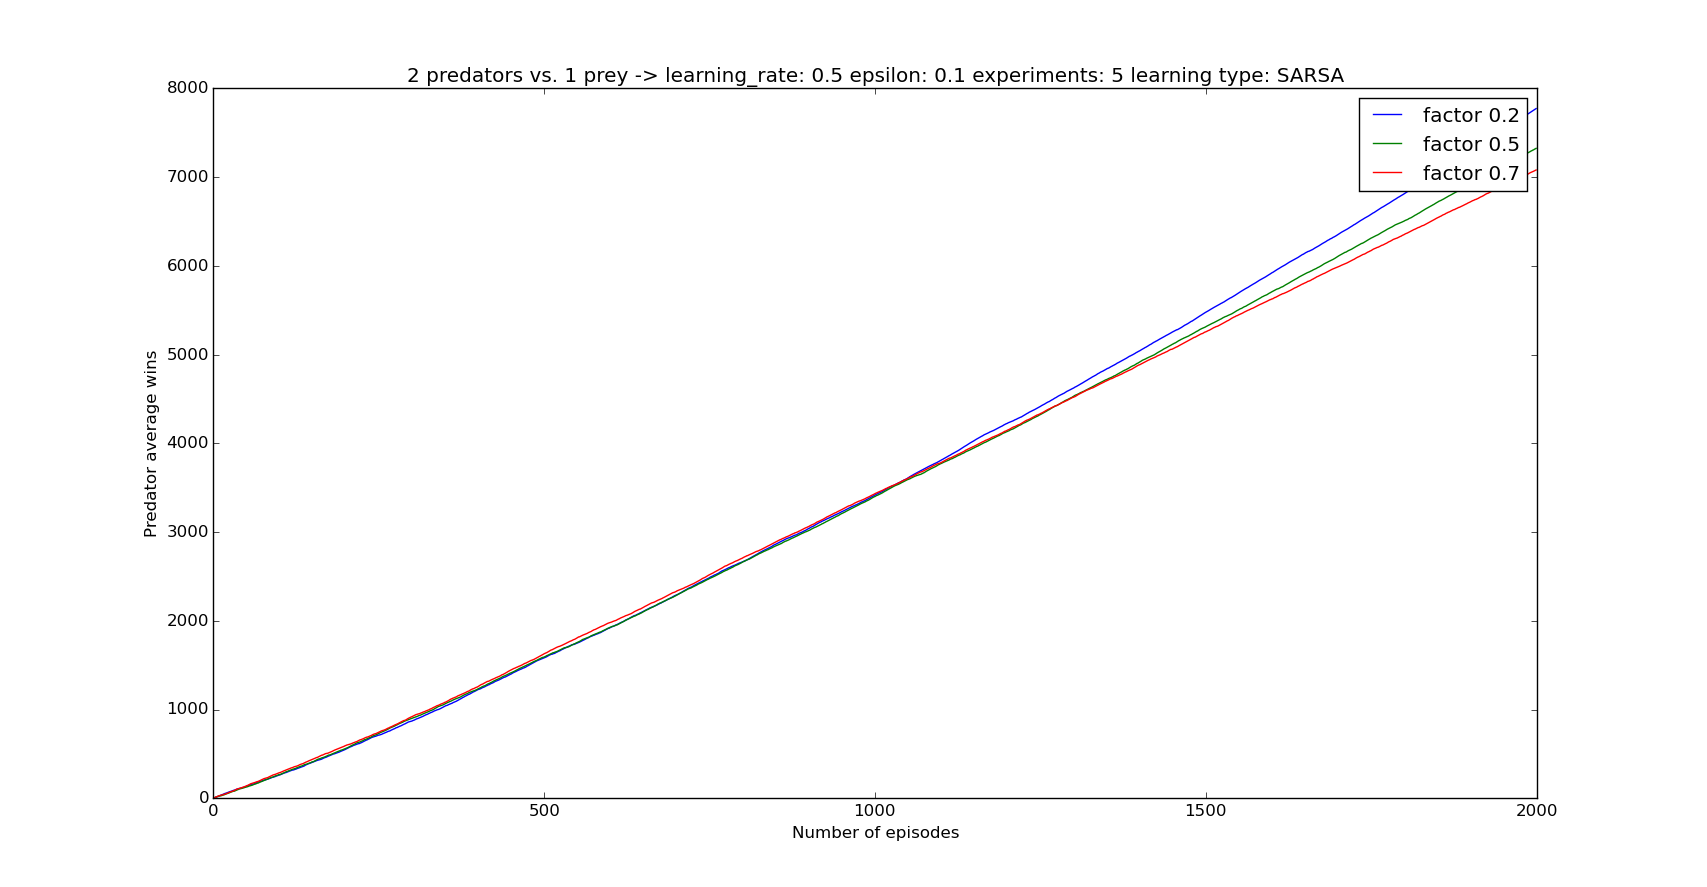
\includegraphics[scale=0.3]{2_predators_discount_factor_SARSA}
	\captionof{figure}{Independent SARSA: 2 predators vs. 1 prey, discount factor}
\end{center}

Again, the immediate reward shows to be important. It has been mentioned several times that SARSA is a careful algorithm, as it collects rewards during learning. Independent Q-learning yields similar results, confirming the theory that introducing a negative reward into the game makes the immediate reward more important.

\begin{table}[H]
\begin{center}
\begin{tabular}{| l | l | l | l | l |}
\hline
\parbox{2cm}{\textbf{$\epsilon$-rate}} & \parbox{2cm}{\textbf{Avg wins \\ (first 100)}} & \parbox{2cm}{\textbf{Avg losses \\ (first 100)}} & \parbox{2cm}{\textbf{Avg wins \\ (last 100)}} & \parbox{2cm}{\textbf{Avg losses \\ (last 100)}} \\
\hline
\textbf{0.2} & 52 & 47 & 95 & 3 \\
\hline
\textbf{0.5} & 53 & 46 & 80 & 18 \\
\hline
\textbf{0.7} & 57 & 42 & 71 & 27 \\
\hline
\end{tabular}
\caption{Average \# wins and losses by the predators with varying discount factors}
\end{center}
\end{table}

The previous conclusions are supported by the table. However, it is interesting to note that keeping into account the immediate reward yields significantly better results than seen before. Winning games 95\% of the time, on average, is highly successful. This means that even when the predators are exploring new paths, the predators hardly ever bump into one another. These are excellent results for any algorithm, let alone an on-policy algorithm.

\subsubsection{$\epsilon$-greedy action selection}
\begin{center}
	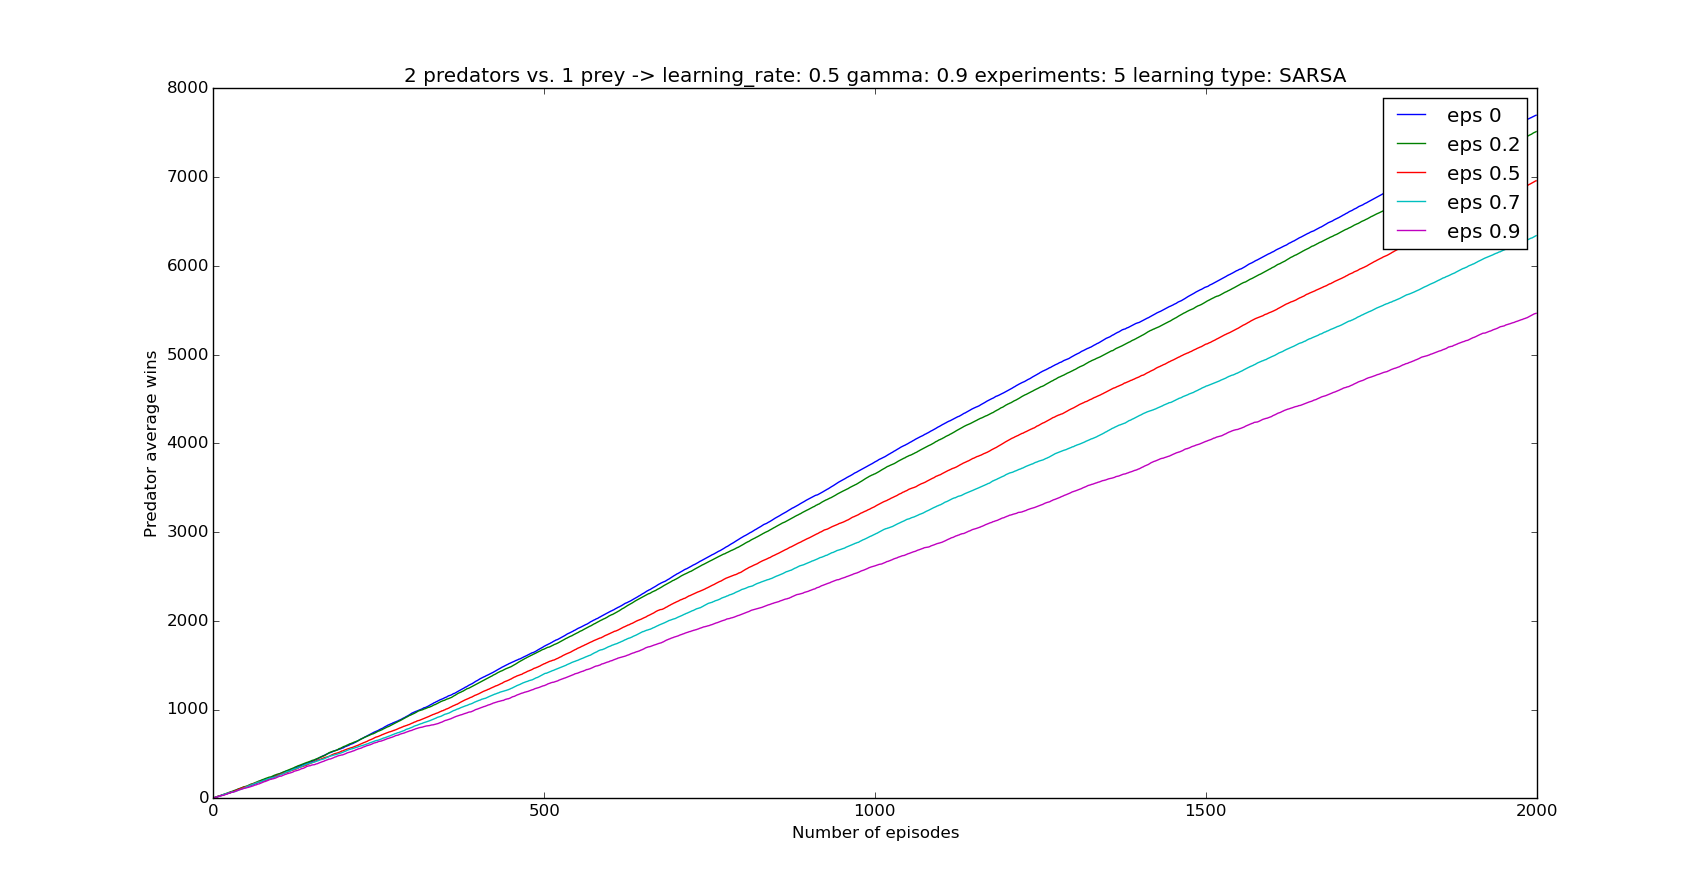
\includegraphics[scale=0.3]{2_predators_epsilon_SARSA}
	\captionof{figure}{Independent SARSA: 2 predators vs. 1 prey, $\epsilon$-greedy action selection}
\end{center}

The graph shows that low exploration leads to the best results. Again, this is to be expected as exploration most likely will lead to predators bumping into one another.

\begin{table}[H]
\begin{center}
\begin{tabular}{| l | l | l | l | l |}
\hline
\parbox{2cm}{\textbf{$\epsilon$-rate}} & \parbox{2cm}{\textbf{Avg wins \\ (first 100)}} & \parbox{2cm}{\textbf{Avg losses \\ (first 100)}} & \parbox{2cm}{\textbf{Avg wins \\ (last 100)}} & \parbox{2cm}{\textbf{Avg losses \\ (last 100)}} \\
\hline
\textbf{0} & 54 & 45 & 74 & 24 \\
\hline
\textbf{0.2} & 55 & 45 & 74 & 24 \\
\hline
\textbf{0.5} & 53 & 47 & 73 & 25 \\
\hline
\textbf{0.7} & 51 & 48 & 66 & 32 \\
\hline
\textbf{0.9} & 48 & 51 & 57 & 41 \\
\hline
\end{tabular}
\caption{Average \# wins and losses by the predators with varying $\epsilon$-rates}
\end{center}
\end{table}

The table confirms almost what the graph shows. Where the graph shows better results for an absolutely greedy action selection, the table shows that the results over the last 100 runs are exactly the same.  This will lead to trying to catch the prey in the beginning, but exploring other paths to the prey while avoiding other predators is also important. This can help the predators significantly in the future. However, exploration is needed. Therefore, lowering the learning rate over time will help the predators best. This confirms the theory that the learning rate must be lowered in order to yield best results.

\subsection{Minimax Q-learning}
\pagebreak


\section{Conclusion}
This section discusses the conclusions drawn from the analysis. %This report has discussed independent multi-agent learning as well as minimax learning in as zero-sum game.

\subsection{Independent learning}
Independent learning was performed in two different ways: Q-learning and SARSA. When more than 2 predators enter the grid, the predators lose the game more often than the prey. This is to be expected as the agents learn independently from one another. Though all agents act on what is best for them, they do not work together. Therefore, all agents must learn each others behaviour before being able to catch the prey without bumping into another predator. This takes very long and even then it is not certain that the predators will catch the prey. As all agents learn each others policies, the prey will also learn what the predators will do and may trick them into bumping into one another.

\subsubsection{Parameter settings}
Parameters settings for both algorithms were tested. 

\subsection{Minimax Q-learning}
Draw thine conclusions and place them here. Oh Romeo, Romeo. Wherefore art thou Romeo? :'(
\pagebreak


\section{Future work}
This section contains information about improvements in the future

\subsection{State space encoding}
It has shown that the state space encoding has improved the performance of the program. However, in order to run tests with four predators on one grid, a smarter encoding is necessary. With a smarter state space encoding, it will be possible to run the program with up to four predators and this research can be completed. The smarter state space encoding will also allow multiple experiments to be run on grids with three or more predators. One possible form of automatic state space encoding at bit level is Kanerva coding\cite{wu2009function}. Kanerva coding compares state-action pairs at a bit level and chooses whichever action looks similar to this. This, itself leads to a smaller state space and an executable program.

\subsection{Grid size}
All the tests were performed on an 11x11 grid. As it is believed that the predators bump into each other so much because the grid is small, it is interesting to see how all agents learn on a larger grid. As stated before, this will significantly increase the state space of the implementation, leading to slow computation. In order to perform these tests, it is imperative to come up with smarter state space encoding. Then these tests can be executed and the effects of these learning algorithms can be evaluated.

\subsection{Communication-based greedy role assignment}
In order to prevent the predators from bumping into one another, communication-based greedy role assignment can me implemented. In this algorithm, cooperating agents get roles assigned. In this case, whichever predator is closest to the prey will get the role of "hunter" and each predator knows their own role as well as the roles of the other predators. The predators that are further away from the prey will get the role of "idle". This gives the "hunter" permission to catch the prey. This will reduce the chances of the predators bumping into one another.

\subsection{WoLF Hill-Climbing}
All types of learning implemented, thus far, will become predictable after convergence. By implementing Win-or-Learn-Fast Hill Climbing, this can be prevented. This algorithm has a variable learning rate. As the name suggests, when the agent wins it hardly learns. When the agents loses, it learns quickly. This is all adjusted by setting the learning rate. As the grid is small and toroidal and it can contain up to four cooperating agents, it is interesting to see what decisions the agents will make.

\subsection{Friend-or-Foe Q-learning}
Another type of Q-learning algorithm is Friend-or-Foe Q-learning\cite{littman2001friend}. This algorithm is an extension of the Minimax-Q algorithm. It takes into account different types of opponent agents: 'friend' and 'foe'. A coordination equilibria is found with a 'friend' agent, while a adversarial equilibria is found with a 'foe' agent. This algorithm could be implemented by identifying the other predators as 'friend' and the prey as 'foe'. This will increase the coordination between predators and decrease the chances of the predators bumping into one another.
\pagebreak


\section{Files attached}

\begin{itemize}
\item newstate.py
\item agents\_new.py
\item other\_objects.py
\item helpers.py \ldots
\end{itemize}


\section{Sources}

% TODO Update the bibliography according to the new assignment
\nocite{*}
\printbibliography


\begin{comment}
\bibliography{bibliography}
\bibliographystyle{plain}
\begin{itemize}
	\item [1] Barto and Sutton (http://webdocs.cs.ualberta.ca/~sutton/book/the-book.html) \ldots
\end{itemize}
\end{comment}


\end{document}